% Created by tikzDevice version 0.12.6 on 2026-08-08 13:32:29
% !TEX encoding = UTF-8 Unicode
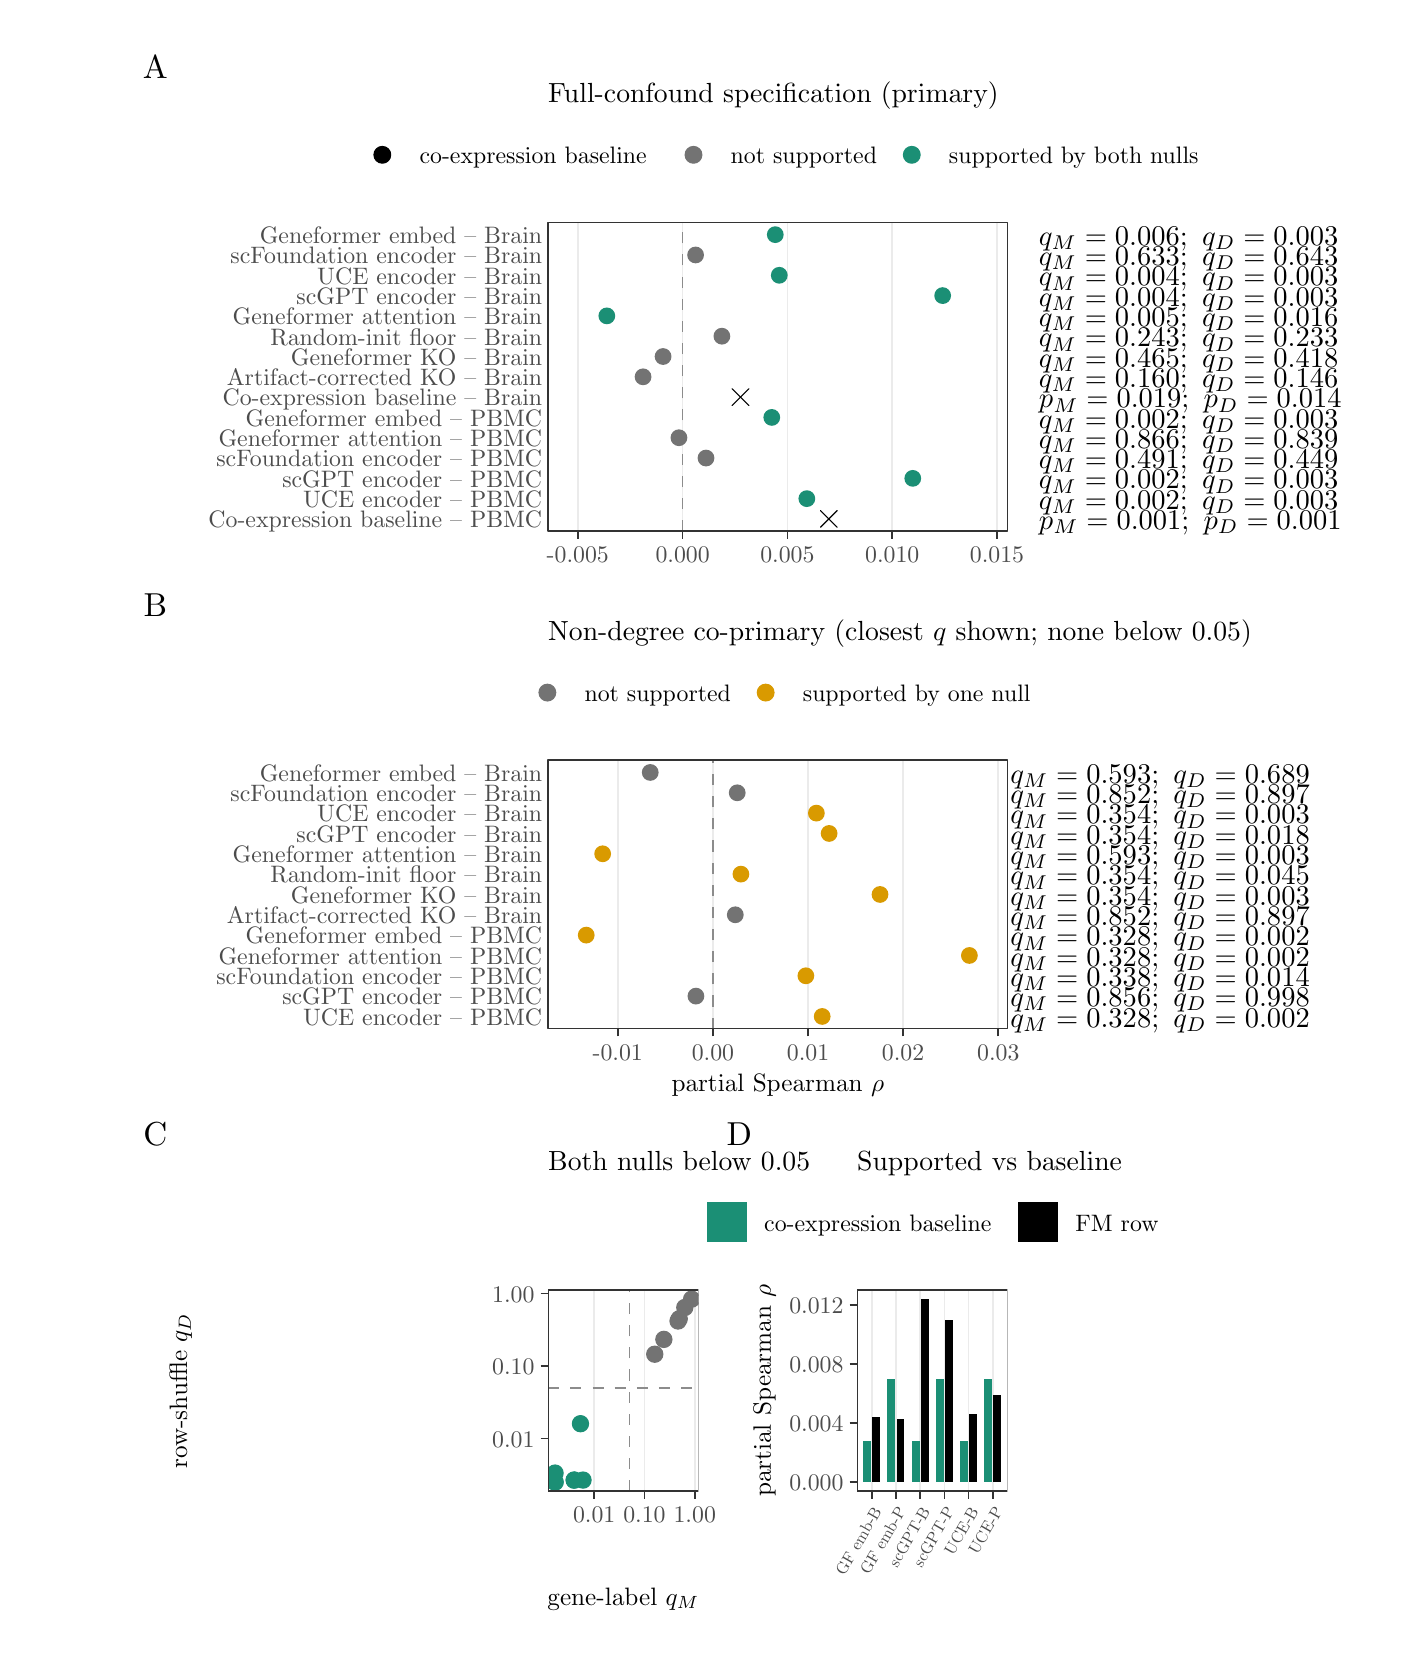
\begin{tikzpicture}[x=1pt,y=1pt]
\definecolor{fillColor}{RGB}{255,255,255}
\path[use as bounding box,fill=fillColor,fill opacity=0.00] (0,0) rectangle (491.44,578.16);
\begin{scope}
\path[clip] (  0.00,  0.00) rectangle (491.44,578.16);
\definecolor{drawColor}{RGB}{255,255,255}
\definecolor{fillColor}{RGB}{255,255,255}

\path[draw=drawColor,line width= 0.6pt,line join=round,line cap=round,fill=fillColor] (  0.00, -0.00) rectangle (491.44,578.16);
\end{scope}
\begin{scope}
\path[clip] (  4.00,379.84) rectangle (485.44,574.16);
\definecolor{drawColor}{RGB}{255,255,255}
\definecolor{fillColor}{RGB}{255,255,255}

\path[draw=drawColor,line width= 0.6pt,line join=round,line cap=round,fill=fillColor] (  4.00,379.84) rectangle (485.44,574.16);
\end{scope}
\begin{scope}
\path[clip] (  4.00,188.43) rectangle (485.44,379.84);
\definecolor{drawColor}{RGB}{255,255,255}
\definecolor{fillColor}{RGB}{255,255,255}

\path[draw=drawColor,line width= 0.6pt,line join=round,line cap=round,fill=fillColor] (  4.00,188.43) rectangle (485.44,379.84);
\end{scope}
\begin{scope}
\path[clip] (  0.00,  0.00) rectangle (491.44,578.16);
\definecolor{fillColor}{RGB}{255,255,255}

\path[fill=fillColor] (188.10,396.23) rectangle (354.02,507.76);
\definecolor{drawColor}{gray}{0.92}

\path[draw=drawColor,line width= 0.6pt,line join=round] (198.79,396.23) --
	(198.79,507.76);

\path[draw=drawColor,line width= 0.6pt,line join=round] (236.66,396.23) --
	(236.66,507.76);

\path[draw=drawColor,line width= 0.6pt,line join=round] (274.53,396.23) --
	(274.53,507.76);

\path[draw=drawColor,line width= 0.6pt,line join=round] (312.40,396.23) --
	(312.40,507.76);

\path[draw=drawColor,line width= 0.6pt,line join=round] (350.26,396.23) --
	(350.26,507.76);
\definecolor{drawColor}{gray}{0.55}

\path[draw=drawColor,line width= 0.6pt,dash pattern=on 4pt off 4pt ,line join=round] (236.66,396.23) -- (236.66,507.76);
\definecolor{fillColor}{RGB}{27,143,117}

\path[fill=fillColor] (270.14,503.36) circle (  3.03);
\definecolor{fillColor}{gray}{0.45}

\path[fill=fillColor] (241.35,496.02) circle (  3.03);
\definecolor{fillColor}{RGB}{27,143,117}

\path[fill=fillColor] (271.59,488.68) circle (  3.03);

\path[fill=fillColor] (330.63,481.34) circle (  3.03);

\path[fill=fillColor] (209.28,474.01) circle (  3.03);
\definecolor{fillColor}{gray}{0.45}

\path[fill=fillColor] (250.85,466.67) circle (  3.03);

\path[fill=fillColor] (229.60,459.33) circle (  3.03);

\path[fill=fillColor] (222.37,451.99) circle (  3.03);
\definecolor{drawColor}{RGB}{0,0,0}

\path[draw=drawColor,line width= 0.4pt,line join=round,line cap=round] (254.53,441.62) -- (260.60,447.69);

\path[draw=drawColor,line width= 0.4pt,line join=round,line cap=round] (254.53,447.69) -- (260.60,441.62);
\definecolor{fillColor}{RGB}{27,143,117}

\path[fill=fillColor] (268.88,437.32) circle (  3.03);
\definecolor{fillColor}{gray}{0.45}

\path[fill=fillColor] (235.33,429.98) circle (  3.03);

\path[fill=fillColor] (245.11,422.64) circle (  3.03);
\definecolor{fillColor}{RGB}{27,143,117}

\path[fill=fillColor] (319.83,415.30) circle (  3.03);

\path[fill=fillColor] (281.55,407.97) circle (  3.03);

\path[draw=drawColor,line width= 0.4pt,line join=round,line cap=round] (286.45,397.60) -- (292.52,403.66);

\path[draw=drawColor,line width= 0.4pt,line join=round,line cap=round] (286.45,403.66) -- (292.52,397.60);

\node[text=drawColor,anchor=base west,inner sep=0pt, outer sep=0pt, scale=  1.03] at (365.41,499.53) {$q_M=0.006;\ q_D=0.003$};

\node[text=drawColor,anchor=base west,inner sep=0pt, outer sep=0pt, scale=  1.03] at (365.41,492.19) {$q_M=0.633;\ q_D=0.643$};

\node[text=drawColor,anchor=base west,inner sep=0pt, outer sep=0pt, scale=  1.03] at (365.41,484.85) {$q_M=0.004;\ q_D=0.003$};

\node[text=drawColor,anchor=base west,inner sep=0pt, outer sep=0pt, scale=  1.03] at (365.41,477.51) {$q_M=0.004;\ q_D=0.003$};

\node[text=drawColor,anchor=base west,inner sep=0pt, outer sep=0pt, scale=  1.03] at (365.41,470.18) {$q_M=0.005;\ q_D=0.016$};

\node[text=drawColor,anchor=base west,inner sep=0pt, outer sep=0pt, scale=  1.03] at (365.41,462.84) {$q_M=0.243;\ q_D=0.233$};

\node[text=drawColor,anchor=base west,inner sep=0pt, outer sep=0pt, scale=  1.03] at (365.41,455.50) {$q_M=0.465;\ q_D=0.418$};

\node[text=drawColor,anchor=base west,inner sep=0pt, outer sep=0pt, scale=  1.03] at (365.41,448.16) {$q_M=0.160;\ q_D=0.146$};

\node[text=drawColor,anchor=base west,inner sep=0pt, outer sep=0pt, scale=  1.03] at (365.41,440.82) {$p_M=0.019;\ p_D=0.014$};

\node[text=drawColor,anchor=base west,inner sep=0pt, outer sep=0pt, scale=  1.03] at (365.41,433.49) {$q_M=0.002;\ q_D=0.003$};

\node[text=drawColor,anchor=base west,inner sep=0pt, outer sep=0pt, scale=  1.03] at (365.41,426.15) {$q_M=0.866;\ q_D=0.839$};

\node[text=drawColor,anchor=base west,inner sep=0pt, outer sep=0pt, scale=  1.03] at (365.41,418.81) {$q_M=0.491;\ q_D=0.449$};

\node[text=drawColor,anchor=base west,inner sep=0pt, outer sep=0pt, scale=  1.03] at (365.41,411.47) {$q_M=0.002;\ q_D=0.003$};

\node[text=drawColor,anchor=base west,inner sep=0pt, outer sep=0pt, scale=  1.03] at (365.41,404.14) {$q_M=0.002;\ q_D=0.003$};

\node[text=drawColor,anchor=base west,inner sep=0pt, outer sep=0pt, scale=  1.03] at (365.41,396.80) {$p_M=0.001;\ p_D=0.001$};
\definecolor{drawColor}{gray}{0.20}

\path[draw=drawColor,line width= 0.6pt,line join=round,line cap=round] (188.10,396.23) rectangle (354.02,507.76);
\end{scope}
\begin{scope}
\path[clip] (  0.00,  0.00) rectangle (491.44,578.16);
\definecolor{drawColor}{gray}{0.30}

\node[text=drawColor,anchor=base east,inner sep=0pt, outer sep=0pt, scale=  0.86] at (185.90,397.43) {Co-expression baseline -- PBMC};

\node[text=drawColor,anchor=base east,inner sep=0pt, outer sep=0pt, scale=  0.86] at (185.90,404.77) {UCE encoder -- PBMC};

\node[text=drawColor,anchor=base east,inner sep=0pt, outer sep=0pt, scale=  0.86] at (185.90,412.11) {scGPT encoder -- PBMC};

\node[text=drawColor,anchor=base east,inner sep=0pt, outer sep=0pt, scale=  0.86] at (185.90,419.45) {scFoundation encoder -- PBMC};

\node[text=drawColor,anchor=base east,inner sep=0pt, outer sep=0pt, scale=  0.86] at (185.90,426.78) {Geneformer attention -- PBMC};

\node[text=drawColor,anchor=base east,inner sep=0pt, outer sep=0pt, scale=  0.86] at (185.90,434.12) {Geneformer embed -- PBMC};

\node[text=drawColor,anchor=base east,inner sep=0pt, outer sep=0pt, scale=  0.86] at (185.90,441.46) {Co-expression baseline -- Brain};

\node[text=drawColor,anchor=base east,inner sep=0pt, outer sep=0pt, scale=  0.86] at (185.90,448.80) {Artifact-corrected KO -- Brain};

\node[text=drawColor,anchor=base east,inner sep=0pt, outer sep=0pt, scale=  0.86] at (185.90,456.13) {Geneformer KO -- Brain};

\node[text=drawColor,anchor=base east,inner sep=0pt, outer sep=0pt, scale=  0.86] at (185.90,463.47) {Random-init floor -- Brain};

\node[text=drawColor,anchor=base east,inner sep=0pt, outer sep=0pt, scale=  0.86] at (185.90,470.81) {Geneformer attention -- Brain};

\node[text=drawColor,anchor=base east,inner sep=0pt, outer sep=0pt, scale=  0.86] at (185.90,478.15) {scGPT encoder -- Brain};

\node[text=drawColor,anchor=base east,inner sep=0pt, outer sep=0pt, scale=  0.86] at (185.90,485.49) {UCE encoder -- Brain};

\node[text=drawColor,anchor=base east,inner sep=0pt, outer sep=0pt, scale=  0.86] at (185.90,492.82) {scFoundation encoder -- Brain};

\node[text=drawColor,anchor=base east,inner sep=0pt, outer sep=0pt, scale=  0.86] at (185.90,500.16) {Geneformer embed -- Brain};
\end{scope}
\begin{scope}
\path[clip] (  0.00,  0.00) rectangle (491.44,578.16);
\definecolor{drawColor}{gray}{0.20}

\path[draw=drawColor,line width= 0.6pt,line join=round] (198.79,393.48) --
	(198.79,396.23);

\path[draw=drawColor,line width= 0.6pt,line join=round] (236.66,393.48) --
	(236.66,396.23);

\path[draw=drawColor,line width= 0.6pt,line join=round] (274.53,393.48) --
	(274.53,396.23);

\path[draw=drawColor,line width= 0.6pt,line join=round] (312.40,393.48) --
	(312.40,396.23);

\path[draw=drawColor,line width= 0.6pt,line join=round] (350.26,393.48) --
	(350.26,396.23);
\end{scope}
\begin{scope}
\path[clip] (  0.00,  0.00) rectangle (491.44,578.16);
\definecolor{drawColor}{gray}{0.30}

\node[text=drawColor,anchor=base,inner sep=0pt, outer sep=0pt, scale=  0.86] at (198.79,384.88) {-0.005};

\node[text=drawColor,anchor=base,inner sep=0pt, outer sep=0pt, scale=  0.86] at (236.66,384.88) {0.000};

\node[text=drawColor,anchor=base,inner sep=0pt, outer sep=0pt, scale=  0.86] at (274.53,384.88) {0.005};

\node[text=drawColor,anchor=base,inner sep=0pt, outer sep=0pt, scale=  0.86] at (312.40,384.88) {0.010};

\node[text=drawColor,anchor=base,inner sep=0pt, outer sep=0pt, scale=  0.86] at (350.26,384.88) {0.015};
\end{scope}
\begin{scope}
\path[clip] (  0.00,  0.00) rectangle (491.44,578.16);
\definecolor{fillColor}{RGB}{255,255,255}

\path[fill=fillColor] (114.70,518.76) rectangle (427.42,545.66);
\end{scope}
\begin{scope}
\path[clip] (  0.00,  0.00) rectangle (491.44,578.16);
\definecolor{fillColor}{RGB}{255,255,255}

\path[fill=fillColor] (120.20,524.26) rectangle (136.10,540.16);
\definecolor{drawColor}{RGB}{0,0,0}
\definecolor{fillColor}{RGB}{0,0,0}

\path[draw=drawColor,line width= 0.4pt,line join=round,line cap=round,fill=fillColor] (128.15,532.21) circle (  3.03);
\end{scope}
\begin{scope}
\path[clip] (  0.00,  0.00) rectangle (491.44,578.16);
\definecolor{fillColor}{RGB}{255,255,255}

\path[fill=fillColor] (232.64,524.26) rectangle (248.54,540.16);
\definecolor{drawColor}{gray}{0.45}
\definecolor{fillColor}{gray}{0.45}

\path[draw=drawColor,line width= 0.4pt,line join=round,line cap=round,fill=fillColor] (240.59,532.21) circle (  3.03);
\end{scope}
\begin{scope}
\path[clip] (  0.00,  0.00) rectangle (491.44,578.16);
\definecolor{fillColor}{RGB}{255,255,255}

\path[fill=fillColor] (311.52,524.26) rectangle (327.42,540.16);
\definecolor{drawColor}{RGB}{27,143,117}
\definecolor{fillColor}{RGB}{27,143,117}

\path[draw=drawColor,line width= 0.4pt,line join=round,line cap=round,fill=fillColor] (319.47,532.21) circle (  3.03);
\end{scope}
\begin{scope}
\path[clip] (  0.00,  0.00) rectangle (491.44,578.16);
\definecolor{drawColor}{RGB}{0,0,0}

\node[text=drawColor,anchor=base west,inner sep=0pt, outer sep=0pt, scale=  0.86] at (141.60,529.01) {co-expression baseline};
\end{scope}
\begin{scope}
\path[clip] (  0.00,  0.00) rectangle (491.44,578.16);
\definecolor{drawColor}{RGB}{0,0,0}

\node[text=drawColor,anchor=base west,inner sep=0pt, outer sep=0pt, scale=  0.86] at (254.04,529.01) {not supported};
\end{scope}
\begin{scope}
\path[clip] (  0.00,  0.00) rectangle (491.44,578.16);
\definecolor{drawColor}{RGB}{0,0,0}

\node[text=drawColor,anchor=base west,inner sep=0pt, outer sep=0pt, scale=  0.86] at (332.92,529.01) {supported by both nulls};
\end{scope}
\begin{scope}
\path[clip] (  0.00,  0.00) rectangle (491.44,578.16);
\definecolor{drawColor}{RGB}{0,0,0}

\node[text=drawColor,anchor=base west,inner sep=0pt, outer sep=0pt, scale=  1.00] at (188.10,551.03) {Full-confound specification (primary)};
\end{scope}
\begin{scope}
\path[clip] (  0.00,  0.00) rectangle (491.44,578.16);
\definecolor{drawColor}{RGB}{0,0,0}

\node[text=drawColor,anchor=base,inner sep=0pt, outer sep=0pt, scale=  1.20] at ( 46.14,559.86) {A};
\end{scope}
\begin{scope}
\path[clip] (  0.00,  0.00) rectangle (491.44,578.16);
\definecolor{fillColor}{RGB}{255,255,255}

\path[fill=fillColor] (188.10,216.45) rectangle (354.02,313.44);
\definecolor{drawColor}{gray}{0.92}

\path[draw=drawColor,line width= 0.6pt,line join=round] (213.23,216.45) --
	(213.23,313.44);

\path[draw=drawColor,line width= 0.6pt,line join=round] (247.61,216.45) --
	(247.61,313.44);

\path[draw=drawColor,line width= 0.6pt,line join=round] (281.98,216.45) --
	(281.98,313.44);

\path[draw=drawColor,line width= 0.6pt,line join=round] (316.35,216.45) --
	(316.35,313.44);

\path[draw=drawColor,line width= 0.6pt,line join=round] (350.73,216.45) --
	(350.73,313.44);
\definecolor{drawColor}{gray}{0.55}

\path[draw=drawColor,line width= 0.6pt,dash pattern=on 4pt off 4pt ,line join=round] (247.61,216.45) -- (247.61,313.44);
\definecolor{fillColor}{gray}{0.45}

\path[fill=fillColor] (224.96,309.03) circle (  3.03);

\path[fill=fillColor] (256.39,301.68) circle (  3.03);
\definecolor{fillColor}{RGB}{217,154,0}

\path[fill=fillColor] (284.99,294.33) circle (  3.03);

\path[fill=fillColor] (289.60,286.99) circle (  3.03);

\path[fill=fillColor] (207.77,279.64) circle (  3.03);

\path[fill=fillColor] (257.73,272.29) circle (  3.03);

\path[fill=fillColor] (307.99,264.94) circle (  3.03);
\definecolor{fillColor}{gray}{0.45}

\path[fill=fillColor] (255.69,257.60) circle (  3.03);
\definecolor{fillColor}{RGB}{217,154,0}

\path[fill=fillColor] (201.83,250.25) circle (  3.03);

\path[fill=fillColor] (340.29,242.90) circle (  3.03);

\path[fill=fillColor] (281.20,235.55) circle (  3.03);
\definecolor{fillColor}{gray}{0.45}

\path[fill=fillColor] (241.47,228.21) circle (  3.03);
\definecolor{fillColor}{RGB}{217,154,0}

\path[fill=fillColor] (287.10,220.86) circle (  3.03);
\definecolor{drawColor}{RGB}{0,0,0}

\node[text=drawColor,anchor=base west,inner sep=0pt, outer sep=0pt, scale=  1.03] at (355.07,305.20) {$q_M=0.593;\ q_D=0.689$};

\node[text=drawColor,anchor=base west,inner sep=0pt, outer sep=0pt, scale=  1.03] at (355.07,297.85) {$q_M=0.852;\ q_D=0.897$};

\node[text=drawColor,anchor=base west,inner sep=0pt, outer sep=0pt, scale=  1.03] at (355.07,290.50) {$q_M=0.354;\ q_D=0.003$};

\node[text=drawColor,anchor=base west,inner sep=0pt, outer sep=0pt, scale=  1.03] at (355.07,283.16) {$q_M=0.354;\ q_D=0.018$};

\node[text=drawColor,anchor=base west,inner sep=0pt, outer sep=0pt, scale=  1.03] at (355.07,275.81) {$q_M=0.593;\ q_D=0.003$};

\node[text=drawColor,anchor=base west,inner sep=0pt, outer sep=0pt, scale=  1.03] at (355.07,268.46) {$q_M=0.354;\ q_D=0.045$};

\node[text=drawColor,anchor=base west,inner sep=0pt, outer sep=0pt, scale=  1.03] at (355.07,261.11) {$q_M=0.354;\ q_D=0.003$};

\node[text=drawColor,anchor=base west,inner sep=0pt, outer sep=0pt, scale=  1.03] at (355.07,253.77) {$q_M=0.852;\ q_D=0.897$};

\node[text=drawColor,anchor=base west,inner sep=0pt, outer sep=0pt, scale=  1.03] at (355.07,246.42) {$q_M=0.328;\ q_D=0.002$};

\node[text=drawColor,anchor=base west,inner sep=0pt, outer sep=0pt, scale=  1.03] at (355.07,239.07) {$q_M=0.328;\ q_D=0.002$};

\node[text=drawColor,anchor=base west,inner sep=0pt, outer sep=0pt, scale=  1.03] at (355.07,231.72) {$q_M=0.338;\ q_D=0.014$};

\node[text=drawColor,anchor=base west,inner sep=0pt, outer sep=0pt, scale=  1.03] at (355.07,224.38) {$q_M=0.856;\ q_D=0.998$};

\node[text=drawColor,anchor=base west,inner sep=0pt, outer sep=0pt, scale=  1.03] at (355.07,217.03) {$q_M=0.328;\ q_D=0.002$};
\definecolor{drawColor}{gray}{0.20}

\path[draw=drawColor,line width= 0.6pt,line join=round,line cap=round] (188.10,216.45) rectangle (354.02,313.44);
\end{scope}
\begin{scope}
\path[clip] (  0.00,  0.00) rectangle (491.44,578.16);
\definecolor{drawColor}{gray}{0.30}

\node[text=drawColor,anchor=base east,inner sep=0pt, outer sep=0pt, scale=  0.86] at (185.90,217.66) {UCE encoder -- PBMC};

\node[text=drawColor,anchor=base east,inner sep=0pt, outer sep=0pt, scale=  0.86] at (185.90,225.01) {scGPT encoder -- PBMC};

\node[text=drawColor,anchor=base east,inner sep=0pt, outer sep=0pt, scale=  0.86] at (185.90,232.36) {scFoundation encoder -- PBMC};

\node[text=drawColor,anchor=base east,inner sep=0pt, outer sep=0pt, scale=  0.86] at (185.90,239.70) {Geneformer attention -- PBMC};

\node[text=drawColor,anchor=base east,inner sep=0pt, outer sep=0pt, scale=  0.86] at (185.90,247.05) {Geneformer embed -- PBMC};

\node[text=drawColor,anchor=base east,inner sep=0pt, outer sep=0pt, scale=  0.86] at (185.90,254.40) {Artifact-corrected KO -- Brain};

\node[text=drawColor,anchor=base east,inner sep=0pt, outer sep=0pt, scale=  0.86] at (185.90,261.75) {Geneformer KO -- Brain};

\node[text=drawColor,anchor=base east,inner sep=0pt, outer sep=0pt, scale=  0.86] at (185.90,269.09) {Random-init floor -- Brain};

\node[text=drawColor,anchor=base east,inner sep=0pt, outer sep=0pt, scale=  0.86] at (185.90,276.44) {Geneformer attention -- Brain};

\node[text=drawColor,anchor=base east,inner sep=0pt, outer sep=0pt, scale=  0.86] at (185.90,283.79) {scGPT encoder -- Brain};

\node[text=drawColor,anchor=base east,inner sep=0pt, outer sep=0pt, scale=  0.86] at (185.90,291.14) {UCE encoder -- Brain};

\node[text=drawColor,anchor=base east,inner sep=0pt, outer sep=0pt, scale=  0.86] at (185.90,298.48) {scFoundation encoder -- Brain};

\node[text=drawColor,anchor=base east,inner sep=0pt, outer sep=0pt, scale=  0.86] at (185.90,305.83) {Geneformer embed -- Brain};
\end{scope}
\begin{scope}
\path[clip] (  0.00,  0.00) rectangle (491.44,578.16);
\definecolor{drawColor}{gray}{0.20}

\path[draw=drawColor,line width= 0.6pt,line join=round] (213.23,213.70) --
	(213.23,216.45);

\path[draw=drawColor,line width= 0.6pt,line join=round] (247.61,213.70) --
	(247.61,216.45);

\path[draw=drawColor,line width= 0.6pt,line join=round] (281.98,213.70) --
	(281.98,216.45);

\path[draw=drawColor,line width= 0.6pt,line join=round] (316.35,213.70) --
	(316.35,216.45);

\path[draw=drawColor,line width= 0.6pt,line join=round] (350.73,213.70) --
	(350.73,216.45);
\end{scope}
\begin{scope}
\path[clip] (  0.00,  0.00) rectangle (491.44,578.16);
\definecolor{drawColor}{gray}{0.30}

\node[text=drawColor,anchor=base,inner sep=0pt, outer sep=0pt, scale=  0.86] at (213.23,205.11) {-0.01};

\node[text=drawColor,anchor=base,inner sep=0pt, outer sep=0pt, scale=  0.86] at (247.61,205.11) {0.00};

\node[text=drawColor,anchor=base,inner sep=0pt, outer sep=0pt, scale=  0.86] at (281.98,205.11) {0.01};

\node[text=drawColor,anchor=base,inner sep=0pt, outer sep=0pt, scale=  0.86] at (316.35,205.11) {0.02};

\node[text=drawColor,anchor=base,inner sep=0pt, outer sep=0pt, scale=  0.86] at (350.73,205.11) {0.03};
\end{scope}
\begin{scope}
\path[clip] (  0.00,  0.00) rectangle (491.44,578.16);
\definecolor{drawColor}{RGB}{0,0,0}

\node[text=drawColor,anchor=base,inner sep=0pt, outer sep=0pt, scale=  0.91] at (271.06,193.58) {partial Spearman $\rho$};
\end{scope}
\begin{scope}
\path[clip] (  0.00,  0.00) rectangle (491.44,578.16);
\definecolor{fillColor}{RGB}{255,255,255}

\path[fill=fillColor] (174.34,324.44) rectangle (367.78,351.34);
\end{scope}
\begin{scope}
\path[clip] (  0.00,  0.00) rectangle (491.44,578.16);
\definecolor{fillColor}{RGB}{255,255,255}

\path[fill=fillColor] (179.84,329.94) rectangle (195.74,345.84);
\definecolor{drawColor}{gray}{0.45}
\definecolor{fillColor}{gray}{0.45}

\path[draw=drawColor,line width= 0.4pt,line join=round,line cap=round,fill=fillColor] (187.79,337.89) circle (  3.03);
\end{scope}
\begin{scope}
\path[clip] (  0.00,  0.00) rectangle (491.44,578.16);
\definecolor{fillColor}{RGB}{255,255,255}

\path[fill=fillColor] (258.72,329.94) rectangle (274.62,345.84);
\definecolor{drawColor}{RGB}{217,154,0}
\definecolor{fillColor}{RGB}{217,154,0}

\path[draw=drawColor,line width= 0.4pt,line join=round,line cap=round,fill=fillColor] (266.67,337.89) circle (  3.03);
\end{scope}
\begin{scope}
\path[clip] (  0.00,  0.00) rectangle (491.44,578.16);
\definecolor{drawColor}{RGB}{0,0,0}

\node[text=drawColor,anchor=base west,inner sep=0pt, outer sep=0pt, scale=  0.86] at (201.24,334.69) {not supported};
\end{scope}
\begin{scope}
\path[clip] (  0.00,  0.00) rectangle (491.44,578.16);
\definecolor{drawColor}{RGB}{0,0,0}

\node[text=drawColor,anchor=base west,inner sep=0pt, outer sep=0pt, scale=  0.86] at (280.12,334.69) {supported by one null};
\end{scope}
\begin{scope}
\path[clip] (  0.00,  0.00) rectangle (491.44,578.16);
\definecolor{drawColor}{RGB}{0,0,0}

\node[text=drawColor,anchor=base west,inner sep=0pt, outer sep=0pt, scale=  1.00] at (188.10,356.71) {Non-degree co-primary (closest $q$ shown; none below 0.05)};
\end{scope}
\begin{scope}
\path[clip] (  0.00,  0.00) rectangle (491.44,578.16);
\definecolor{drawColor}{RGB}{0,0,0}

\node[text=drawColor,anchor=base,inner sep=0pt, outer sep=0pt, scale=  1.20] at ( 46.14,365.53) {B};
\end{scope}
\begin{scope}
\path[clip] (  4.00,  3.00) rectangle (248.39,188.43);
\definecolor{drawColor}{RGB}{255,255,255}
\definecolor{fillColor}{RGB}{255,255,255}

\path[draw=drawColor,line width= 0.6pt,line join=round,line cap=round,fill=fillColor] (  4.00,  3.00) rectangle (248.39,188.43);
\end{scope}
\begin{scope}
\path[clip] (248.39,  3.00) rectangle (485.44,188.43);
\definecolor{drawColor}{RGB}{255,255,255}
\definecolor{fillColor}{RGB}{255,255,255}

\path[draw=drawColor,line width= 0.6pt,line join=round,line cap=round,fill=fillColor] (248.39,  3.00) rectangle (485.44,188.43);
\end{scope}
\begin{scope}
\path[clip] (188.10, 49.29) rectangle (242.39,122.03);
\definecolor{fillColor}{RGB}{255,255,255}

\path[fill=fillColor] (188.10, 49.29) rectangle (242.39,122.03);
\definecolor{drawColor}{gray}{0.92}

\path[draw=drawColor,line width= 0.6pt,line join=round] (204.71, 49.29) --
	(204.71,122.03);

\path[draw=drawColor,line width= 0.6pt,line join=round] (222.88, 49.29) --
	(222.88,122.03);

\path[draw=drawColor,line width= 0.6pt,line join=round] (241.05, 49.29) --
	(241.05,122.03);
\definecolor{drawColor}{gray}{0.55}

\path[draw=drawColor,line width= 0.6pt,dash pattern=on 4pt off 4pt ,line join=round] (217.41, 49.29) -- (217.41,122.03);

\path[draw=drawColor,line width= 0.6pt,dash pattern=on 4pt off 4pt ,line join=round] (188.10, 86.65) -- (242.39, 86.65);
\definecolor{drawColor}{RGB}{27,143,117}
\definecolor{fillColor}{RGB}{27,143,117}

\path[draw=drawColor,line width= 0.4pt,line join=round,line cap=round,fill=fillColor] (200.68, 53.33) circle (  2.93);
\definecolor{drawColor}{gray}{0.45}
\definecolor{fillColor}{gray}{0.45}

\path[draw=drawColor,line width= 0.4pt,line join=round,line cap=round,fill=fillColor] (237.45,115.69) circle (  2.93);
\definecolor{drawColor}{RGB}{27,143,117}
\definecolor{fillColor}{RGB}{27,143,117}

\path[draw=drawColor,line width= 0.4pt,line join=round,line cap=round,fill=fillColor] (197.48, 53.33) circle (  2.93);

\path[draw=drawColor,line width= 0.4pt,line join=round,line cap=round,fill=fillColor] (197.48, 53.33) circle (  2.93);

\path[draw=drawColor,line width= 0.4pt,line join=round,line cap=round,fill=fillColor] (199.75, 73.70) circle (  2.93);
\definecolor{drawColor}{gray}{0.45}
\definecolor{fillColor}{gray}{0.45}

\path[draw=drawColor,line width= 0.4pt,line join=round,line cap=round,fill=fillColor] (229.88,104.17) circle (  2.93);

\path[draw=drawColor,line width= 0.4pt,line join=round,line cap=round,fill=fillColor] (235.01,110.81) circle (  2.93);

\path[draw=drawColor,line width= 0.4pt,line join=round,line cap=round,fill=fillColor] (226.59, 98.81) circle (  2.93);
\definecolor{drawColor}{RGB}{27,143,117}
\definecolor{fillColor}{RGB}{27,143,117}

\path[draw=drawColor,line width= 0.4pt,line join=round,line cap=round,fill=fillColor] (190.57, 55.86) circle (  2.93);
\definecolor{drawColor}{gray}{0.45}
\definecolor{fillColor}{gray}{0.45}

\path[draw=drawColor,line width= 0.4pt,line join=round,line cap=round,fill=fillColor] (239.92,118.72) circle (  2.93);

\path[draw=drawColor,line width= 0.4pt,line join=round,line cap=round,fill=fillColor] (235.44,111.61) circle (  2.93);
\definecolor{drawColor}{RGB}{27,143,117}
\definecolor{fillColor}{RGB}{27,143,117}

\path[draw=drawColor,line width= 0.4pt,line join=round,line cap=round,fill=fillColor] (190.57, 52.59) circle (  2.93);

\path[draw=drawColor,line width= 0.4pt,line join=round,line cap=round,fill=fillColor] (190.57, 52.59) circle (  2.93);
\definecolor{drawColor}{gray}{0.20}

\path[draw=drawColor,line width= 0.6pt,line join=round,line cap=round] (188.10, 49.29) rectangle (242.39,122.03);
\end{scope}
\begin{scope}
\path[clip] (  0.00,  0.00) rectangle (491.44,578.16);
\definecolor{drawColor}{gray}{0.30}

\node[text=drawColor,anchor=base east,inner sep=0pt, outer sep=0pt, scale=  0.86] at (183.15, 65.16) {0.01};

\node[text=drawColor,anchor=base east,inner sep=0pt, outer sep=0pt, scale=  0.86] at (183.15, 91.34) {0.10};

\node[text=drawColor,anchor=base east,inner sep=0pt, outer sep=0pt, scale=  0.86] at (183.15,117.52) {1.00};
\end{scope}
\begin{scope}
\path[clip] (  0.00,  0.00) rectangle (491.44,578.16);
\definecolor{drawColor}{gray}{0.20}

\path[draw=drawColor,line width= 0.6pt,line join=round] (185.35, 68.36) --
	(188.10, 68.36);

\path[draw=drawColor,line width= 0.6pt,line join=round] (185.35, 94.54) --
	(188.10, 94.54);

\path[draw=drawColor,line width= 0.6pt,line join=round] (185.35,120.72) --
	(188.10,120.72);
\end{scope}
\begin{scope}
\path[clip] (  0.00,  0.00) rectangle (491.44,578.16);
\definecolor{drawColor}{gray}{0.20}

\path[draw=drawColor,line width= 0.6pt,line join=round] (204.71, 46.54) --
	(204.71, 49.29);

\path[draw=drawColor,line width= 0.6pt,line join=round] (222.88, 46.54) --
	(222.88, 49.29);

\path[draw=drawColor,line width= 0.6pt,line join=round] (241.05, 46.54) --
	(241.05, 49.29);
\end{scope}
\begin{scope}
\path[clip] (  0.00,  0.00) rectangle (491.44,578.16);
\definecolor{drawColor}{gray}{0.30}

\node[text=drawColor,anchor=base,inner sep=0pt, outer sep=0pt, scale=  0.86] at (204.71, 37.94) {0.01};

\node[text=drawColor,anchor=base,inner sep=0pt, outer sep=0pt, scale=  0.86] at (222.88, 37.94) {0.10};

\node[text=drawColor,anchor=base,inner sep=0pt, outer sep=0pt, scale=  0.86] at (241.05, 37.94) {1.00};
\end{scope}
\begin{scope}
\path[clip] (  0.00,  0.00) rectangle (491.44,578.16);
\definecolor{drawColor}{RGB}{0,0,0}

\node[text=drawColor,anchor=base,inner sep=0pt, outer sep=0pt, scale=  0.91] at (215.24,  8.16) {gene-label $q_M$};
\end{scope}
\begin{scope}
\path[clip] (  0.00,  0.00) rectangle (491.44,578.16);
\definecolor{drawColor}{RGB}{0,0,0}

\node[text=drawColor,rotate= 90.00,anchor=base,inner sep=0pt, outer sep=0pt, scale=  0.91] at ( 57.61, 85.66) {row-shuffle $q_D$};
\end{scope}
\begin{scope}
\path[clip] (  0.00,  0.00) rectangle (491.44,578.16);
\definecolor{drawColor}{RGB}{0,0,0}

\node[text=drawColor,anchor=base west,inner sep=0pt, outer sep=0pt, scale=  1.00] at (188.10,165.30) {Both nulls below 0.05};
\end{scope}
\begin{scope}
\path[clip] (  0.00,  0.00) rectangle (491.44,578.16);
\definecolor{drawColor}{RGB}{0,0,0}

\node[text=drawColor,anchor=base,inner sep=0pt, outer sep=0pt, scale=  1.20] at ( 46.14,174.12) {C};
\end{scope}
\begin{scope}
\path[clip] (299.74, 49.29) rectangle (354.02,122.03);
\definecolor{fillColor}{RGB}{255,255,255}

\path[fill=fillColor] (299.74, 49.29) rectangle (354.02,122.03);
\definecolor{drawColor}{gray}{0.92}

\path[draw=drawColor,line width= 0.6pt,line join=round] (304.99, 49.29) --
	(304.99,122.03);

\path[draw=drawColor,line width= 0.6pt,line join=round] (313.74, 49.29) --
	(313.74,122.03);

\path[draw=drawColor,line width= 0.6pt,line join=round] (322.50, 49.29) --
	(322.50,122.03);

\path[draw=drawColor,line width= 0.6pt,line join=round] (331.26, 49.29) --
	(331.26,122.03);

\path[draw=drawColor,line width= 0.6pt,line join=round] (340.01, 49.29) --
	(340.01,122.03);

\path[draw=drawColor,line width= 0.6pt,line join=round] (348.77, 49.29) --
	(348.77,122.03);
\definecolor{fillColor}{RGB}{0,0,0}

\path[fill=fillColor] (305.21, 52.59) rectangle (308.05, 76.15);
\definecolor{fillColor}{RGB}{27,143,117}

\path[fill=fillColor] (301.92, 52.59) rectangle (304.77, 67.30);
\definecolor{fillColor}{RGB}{0,0,0}

\path[fill=fillColor] (340.23, 52.59) rectangle (343.08, 77.17);
\definecolor{fillColor}{RGB}{27,143,117}

\path[fill=fillColor] (336.95, 52.59) rectangle (339.79, 67.30);
\definecolor{fillColor}{RGB}{0,0,0}

\path[fill=fillColor] (322.72, 52.59) rectangle (325.56,118.72);
\definecolor{fillColor}{RGB}{27,143,117}

\path[fill=fillColor] (319.44, 52.59) rectangle (322.28, 67.30);
\definecolor{fillColor}{RGB}{0,0,0}

\path[fill=fillColor] (313.96, 52.59) rectangle (316.81, 75.27);
\definecolor{fillColor}{RGB}{27,143,117}

\path[fill=fillColor] (310.68, 52.59) rectangle (313.53, 89.77);
\definecolor{fillColor}{RGB}{0,0,0}

\path[fill=fillColor] (331.47, 52.59) rectangle (334.32,111.12);
\definecolor{fillColor}{RGB}{27,143,117}

\path[fill=fillColor] (328.19, 52.59) rectangle (331.04, 89.77);
\definecolor{fillColor}{RGB}{0,0,0}

\path[fill=fillColor] (348.99, 52.59) rectangle (351.83, 84.18);
\definecolor{fillColor}{RGB}{27,143,117}

\path[fill=fillColor] (345.70, 52.59) rectangle (348.55, 89.77);
\definecolor{drawColor}{gray}{0.20}

\path[draw=drawColor,line width= 0.6pt,line join=round,line cap=round] (299.74, 49.29) rectangle (354.02,122.03);
\end{scope}
\begin{scope}
\path[clip] (  0.00,  0.00) rectangle (491.44,578.16);
\definecolor{drawColor}{gray}{0.30}

\node[text=drawColor,anchor=base east,inner sep=0pt, outer sep=0pt, scale=  0.86] at (294.79, 49.40) {0.000};

\node[text=drawColor,anchor=base east,inner sep=0pt, outer sep=0pt, scale=  0.86] at (294.79, 70.72) {0.004};

\node[text=drawColor,anchor=base east,inner sep=0pt, outer sep=0pt, scale=  0.86] at (294.79, 92.04) {0.008};

\node[text=drawColor,anchor=base east,inner sep=0pt, outer sep=0pt, scale=  0.86] at (294.79,113.35) {0.012};
\end{scope}
\begin{scope}
\path[clip] (  0.00,  0.00) rectangle (491.44,578.16);
\definecolor{drawColor}{gray}{0.20}

\path[draw=drawColor,line width= 0.6pt,line join=round] (296.99, 52.59) --
	(299.74, 52.59);

\path[draw=drawColor,line width= 0.6pt,line join=round] (296.99, 73.91) --
	(299.74, 73.91);

\path[draw=drawColor,line width= 0.6pt,line join=round] (296.99, 95.23) --
	(299.74, 95.23);

\path[draw=drawColor,line width= 0.6pt,line join=round] (296.99,116.55) --
	(299.74,116.55);
\end{scope}
\begin{scope}
\path[clip] (  0.00,  0.00) rectangle (491.44,578.16);
\definecolor{drawColor}{gray}{0.20}

\path[draw=drawColor,line width= 0.6pt,line join=round] (304.99, 46.54) --
	(304.99, 49.29);

\path[draw=drawColor,line width= 0.6pt,line join=round] (313.74, 46.54) --
	(313.74, 49.29);

\path[draw=drawColor,line width= 0.6pt,line join=round] (322.50, 46.54) --
	(322.50, 49.29);

\path[draw=drawColor,line width= 0.6pt,line join=round] (331.26, 46.54) --
	(331.26, 49.29);

\path[draw=drawColor,line width= 0.6pt,line join=round] (340.01, 46.54) --
	(340.01, 49.29);

\path[draw=drawColor,line width= 0.6pt,line join=round] (348.77, 46.54) --
	(348.77, 49.29);
\end{scope}
\begin{scope}
\path[clip] (  0.00,  0.00) rectangle (491.44,578.16);
\definecolor{drawColor}{gray}{0.30}

\node[text=drawColor,rotate= 60.00,anchor=base east,inner sep=0pt, outer sep=0pt, scale=  0.59] at (308.78, 42.15) {GF emb-B};

\node[text=drawColor,rotate= 60.00,anchor=base east,inner sep=0pt, outer sep=0pt, scale=  0.59] at (317.53, 42.15) {GF emb-P};

\node[text=drawColor,rotate= 60.00,anchor=base east,inner sep=0pt, outer sep=0pt, scale=  0.59] at (326.29, 42.15) {scGPT-B};

\node[text=drawColor,rotate= 60.00,anchor=base east,inner sep=0pt, outer sep=0pt, scale=  0.59] at (335.04, 42.15) {scGPT-P};

\node[text=drawColor,rotate= 60.00,anchor=base east,inner sep=0pt, outer sep=0pt, scale=  0.59] at (343.80, 42.15) {UCE-B};

\node[text=drawColor,rotate= 60.00,anchor=base east,inner sep=0pt, outer sep=0pt, scale=  0.59] at (352.55, 42.15) {UCE-P};
\end{scope}
\begin{scope}
\path[clip] (  0.00,  0.00) rectangle (491.44,578.16);
\definecolor{drawColor}{RGB}{0,0,0}

\node[text=drawColor,rotate= 90.00,anchor=base,inner sep=0pt, outer sep=0pt, scale=  0.91] at (268.60, 85.66) {partial Spearman $\rho$};
\end{scope}
\begin{scope}
\path[clip] (  0.00,  0.00) rectangle (491.44,578.16);
\definecolor{fillColor}{RGB}{255,255,255}

\path[fill=fillColor] (239.26,133.03) rectangle (414.50,159.93);
\end{scope}
\begin{scope}
\path[clip] (  0.00,  0.00) rectangle (491.44,578.16);
\definecolor{fillColor}{RGB}{255,255,255}

\path[fill=fillColor] (244.76,138.53) rectangle (260.65,154.43);
\definecolor{fillColor}{RGB}{27,143,117}

\path[fill=fillColor] (245.47,139.24) rectangle (259.94,153.71);
\end{scope}
\begin{scope}
\path[clip] (  0.00,  0.00) rectangle (491.44,578.16);
\definecolor{fillColor}{RGB}{255,255,255}

\path[fill=fillColor] (357.20,138.53) rectangle (373.10,154.43);
\definecolor{fillColor}{RGB}{0,0,0}

\path[fill=fillColor] (357.91,139.24) rectangle (372.39,153.71);
\end{scope}
\begin{scope}
\path[clip] (  0.00,  0.00) rectangle (491.44,578.16);
\definecolor{drawColor}{RGB}{0,0,0}

\node[text=drawColor,anchor=base west,inner sep=0pt, outer sep=0pt, scale=  0.86] at (266.15,143.28) {co-expression baseline};
\end{scope}
\begin{scope}
\path[clip] (  0.00,  0.00) rectangle (491.44,578.16);
\definecolor{drawColor}{RGB}{0,0,0}

\node[text=drawColor,anchor=base west,inner sep=0pt, outer sep=0pt, scale=  0.86] at (378.60,143.28) {FM row};
\end{scope}
\begin{scope}
\path[clip] (  0.00,  0.00) rectangle (491.44,578.16);
\definecolor{drawColor}{RGB}{0,0,0}

\node[text=drawColor,anchor=base west,inner sep=0pt, outer sep=0pt, scale=  1.00] at (299.74,165.30) {Supported vs baseline};
\end{scope}
\begin{scope}
\path[clip] (  0.00,  0.00) rectangle (491.44,578.16);
\definecolor{drawColor}{RGB}{0,0,0}

\node[text=drawColor,anchor=base,inner sep=0pt, outer sep=0pt, scale=  1.20] at (257.13,174.12) {D};
\end{scope}
\end{tikzpicture}
